\documentclass[12pt]{report}
\usepackage[margin=1.25in]{geometry}
\usepackage[hidelinks]{hyperref}
\usepackage{graphicx}
\usepackage{rotating}
\usepackage{forest}
\usepackage{listings}

\renewcommand{\familydefault}{\sfdefault}

\newcommand{\inlinecode}{\texttt}

\begin{document}
\tableofcontents
\chapter{Research}
\section{Related Projects}

After gathering requirements from our client we decided to try and find
applications with a similar design or feature set, to decide on a simple way to
build the overall systems architecture and refine the initial requirement that
we got from the client. However, there did not seem to be much on the market
that matched the clients full description i.e.\ a system at allows a normal
user to tag virtual reality videos, with text, html, audio \ldots, and then
allows them to play those tagged videos back on a mobile device such as the
Samsung Gear VR\@. 

The closest we could find to an app that fulfilled the clients specification was
an application called ``ThingLink'' at
\url{http://demo.thinglink.com/vr-editor} which did most of the tasks that the
client wanted performed but the ability to edit display 360 video comes at a fee of
£125 per user per month which is prohibitively expensive for charity work, as
well as that there is no guaranty that the off-the-shelf software can be
updated to fit all of the clients needs as requirements change. But ThingLink
did give us the idea to create a Client/Server application that would export
custom data files that any client could use. And in the tradition of other
android file formats we decided the best thing to do would be to use a renamed
zip file with a metadata file inside it. Our system however, would improve on
the software by using as many Open Source components as possible in an effort
to reduce our clients maintenance troubles as well as fulfil one of the ethical
requirements that they had given us. 

With that in mind we looked at the VR Player FREE
\url{https://play.google.com/store/apps/details?id=com.vimersiv.vrplayerfree}
for inspiration on how to build an interface and relayed my findings to my
partner Jasper, informing him about the limitations of the Gear VR's input
system and that the interface might need to be made simpler and more
streamlined so as to better show up on the Gear VR\@. VR Player FREE was also
one of the applications that was brought up in meetings as a possible related
project as it did support 360 VR video that the client wanted but it did not
support any tagging features and didn't provide an editor or any equivalent
capability, ruling it out as it did not meet the clients requirements. Our
system however will be different to VR Player FREE as it will have the ability
to display tagged files.

\chapter{Design and Implementation}

\section{Design}

\subsection{System Architecture Diagram}
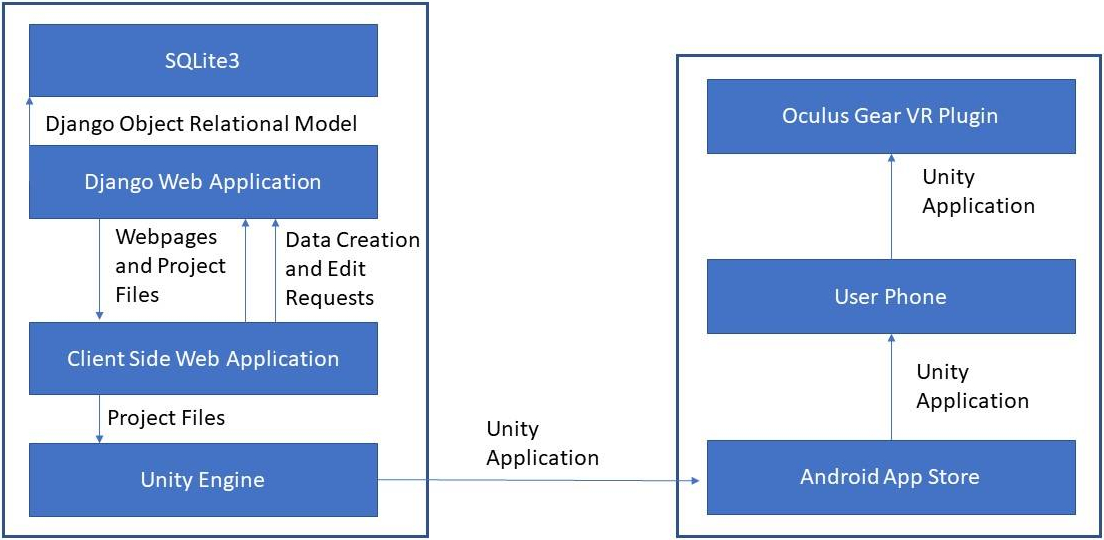
\includegraphics[width=\textwidth]{system_arch}

\begin{description}
    \item [SQLite3] is a simple file-based relational database that works by
        writing all of it's changes into a single db.sqlite3 file. It is would
        used by the application to store all of the project metadata such as
        project-video lists and tagging meta-information. It forms the model
        part of a traditional model-view-controller (MVC) architecture.

    \item [Django Web Application] is a web application framework written in
        python and uses the WSGI (Web Server Gateway Interface) to communicate
        with a webserver to allow it to serve web requests. The application
        will translate the web-requests that it is given, update the database
        and reply with a given HTML response. It forms the controller of the
        MVC architecture.

    \item [Client Side Web Application] is mostly made of HTML and JavaScript
        that is rendered out from templates by the Django app. It provides an
        interface to create/read/update/destroy/export projects/videos/tags as
        required. This forms the view part of a traditional MVC architecture.

    \item [Unity Engine] The Unity Engine is the game engine that we will be
        using to perform all of the cross-platform OpenGL rendering and video
        playing that is necessary to simulate virtual reality and perform 3d
        tagging.

    \item [Android App Store] is a virtual storefront that allows users to
        download and run applications on their Android Phones. 

    \item [User Phone] will run the Unity Application allow the
        user to interact with the VR space, choose which video to play and
        handle the display of all the tags.

    \item [Oculus Gear VR Plugin] is a library that manipulates the Camera in a
        Unity Scene to track with the user's head movements and allow them use
        the Gear VR to look around in 3D space.
\end{description}

\subsection{Site Maps}
All traversals are user driven, two-way, navigation.

\subsubsection{VR Tagging Engine Sitemap}

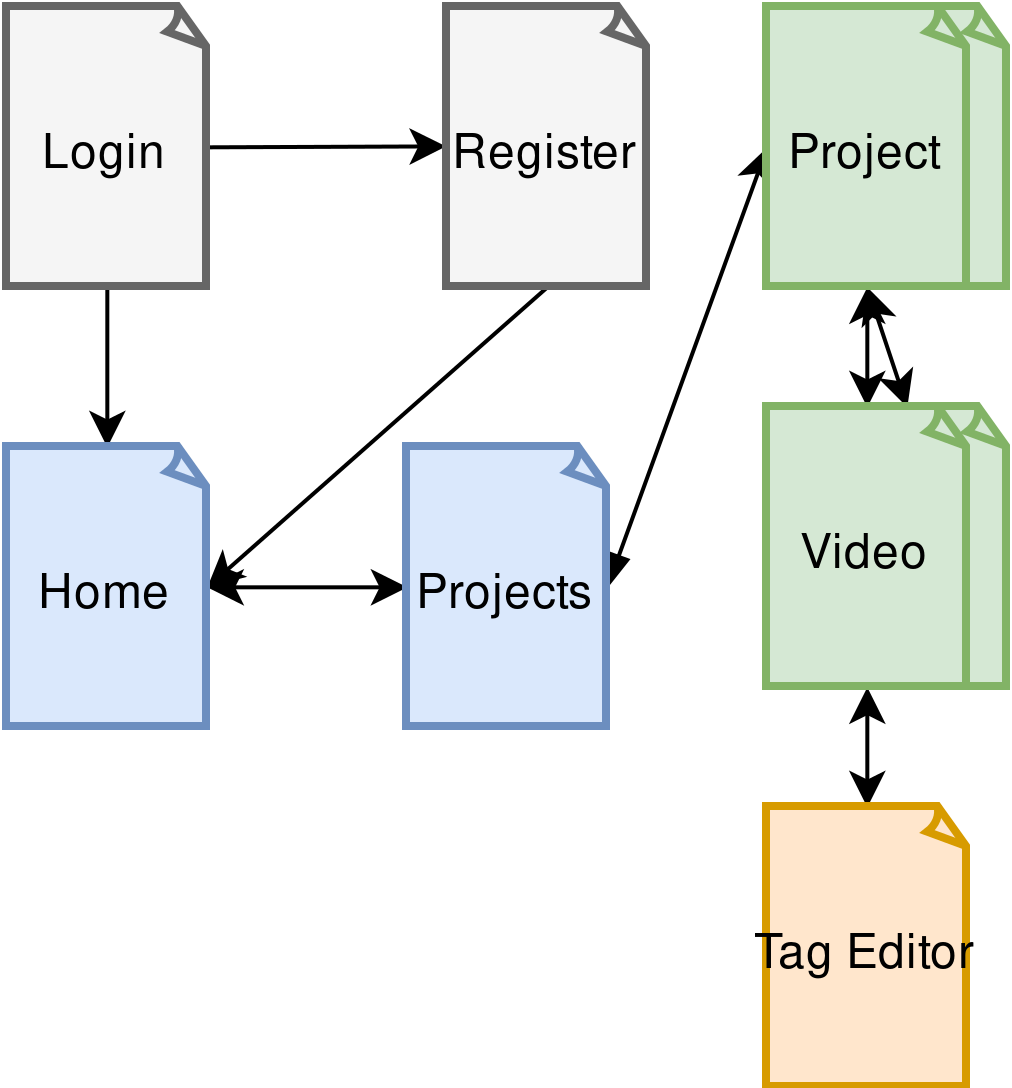
\includegraphics[width=\textwidth]{web_site_map}

\subsubsection{VR Viewer Sitemap}

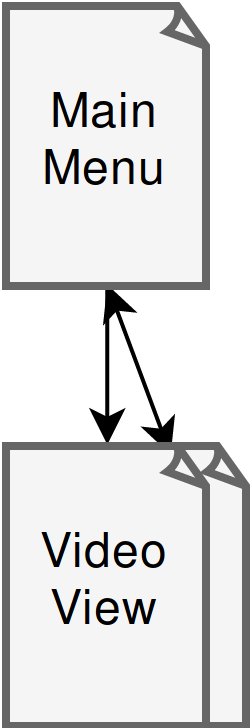
\includegraphics[height=\textwidth]{unity_site_map}

\subsection{Application Structure}
\subsubsection{VR Tagging Engine}
\begin{sideways}
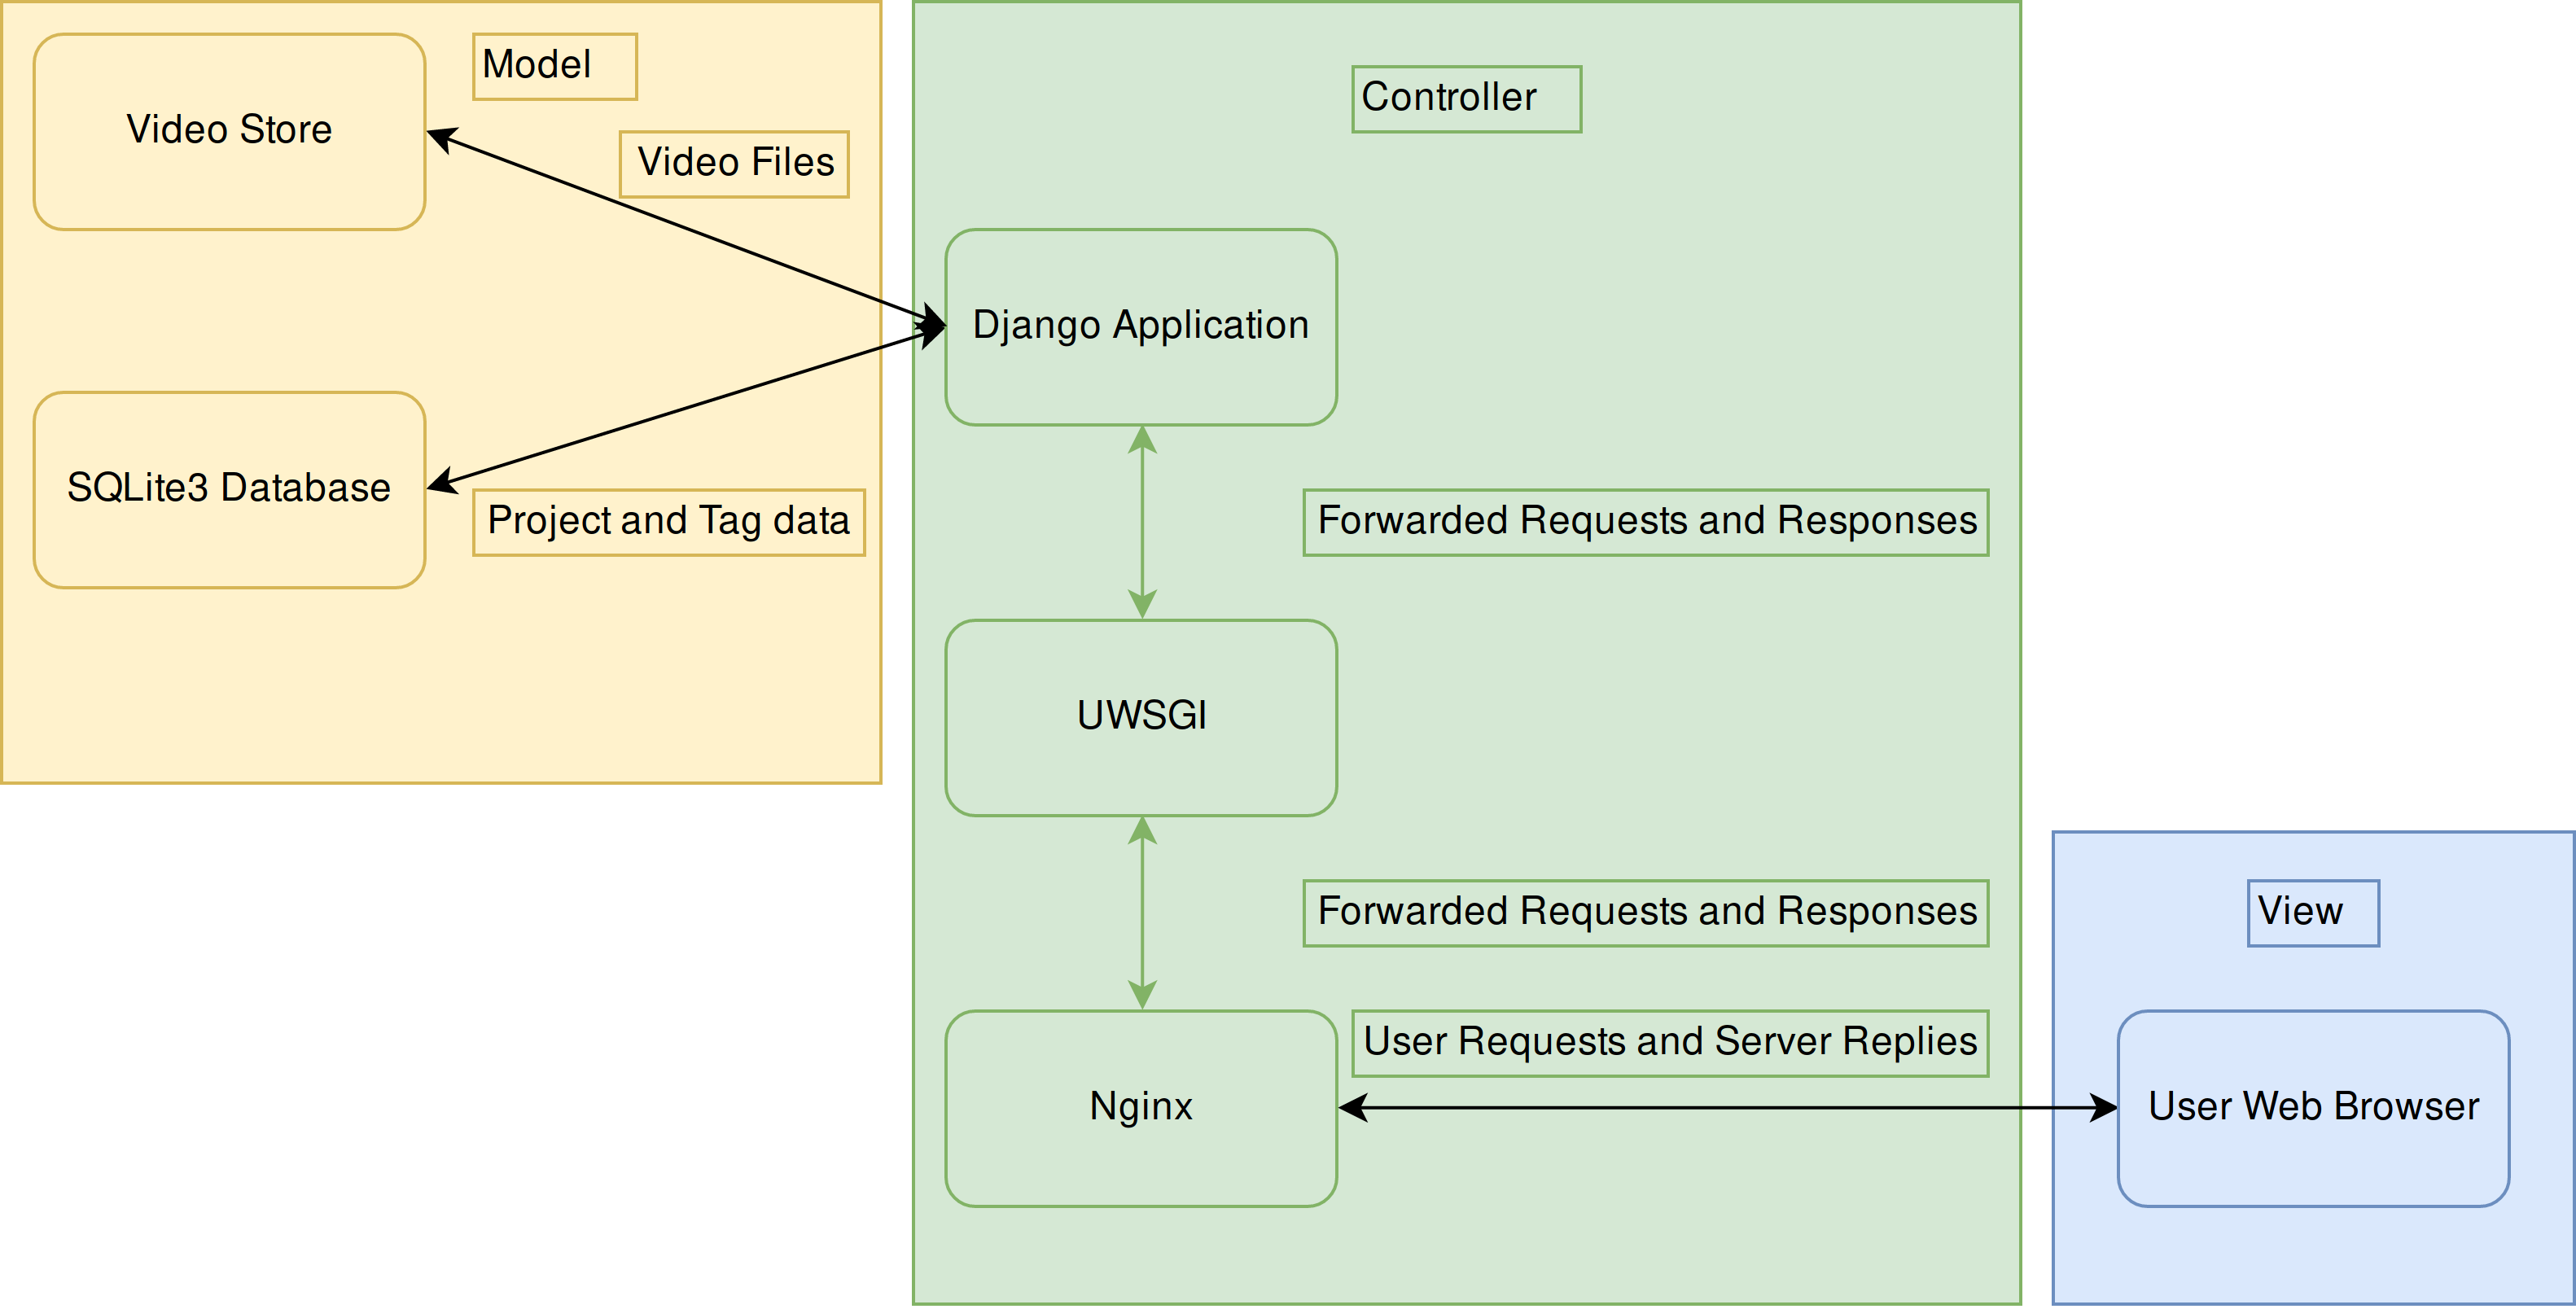
\includegraphics[height=9cm]{application_struct}
\end{sideways}

\subsubsection{VR Viewer}
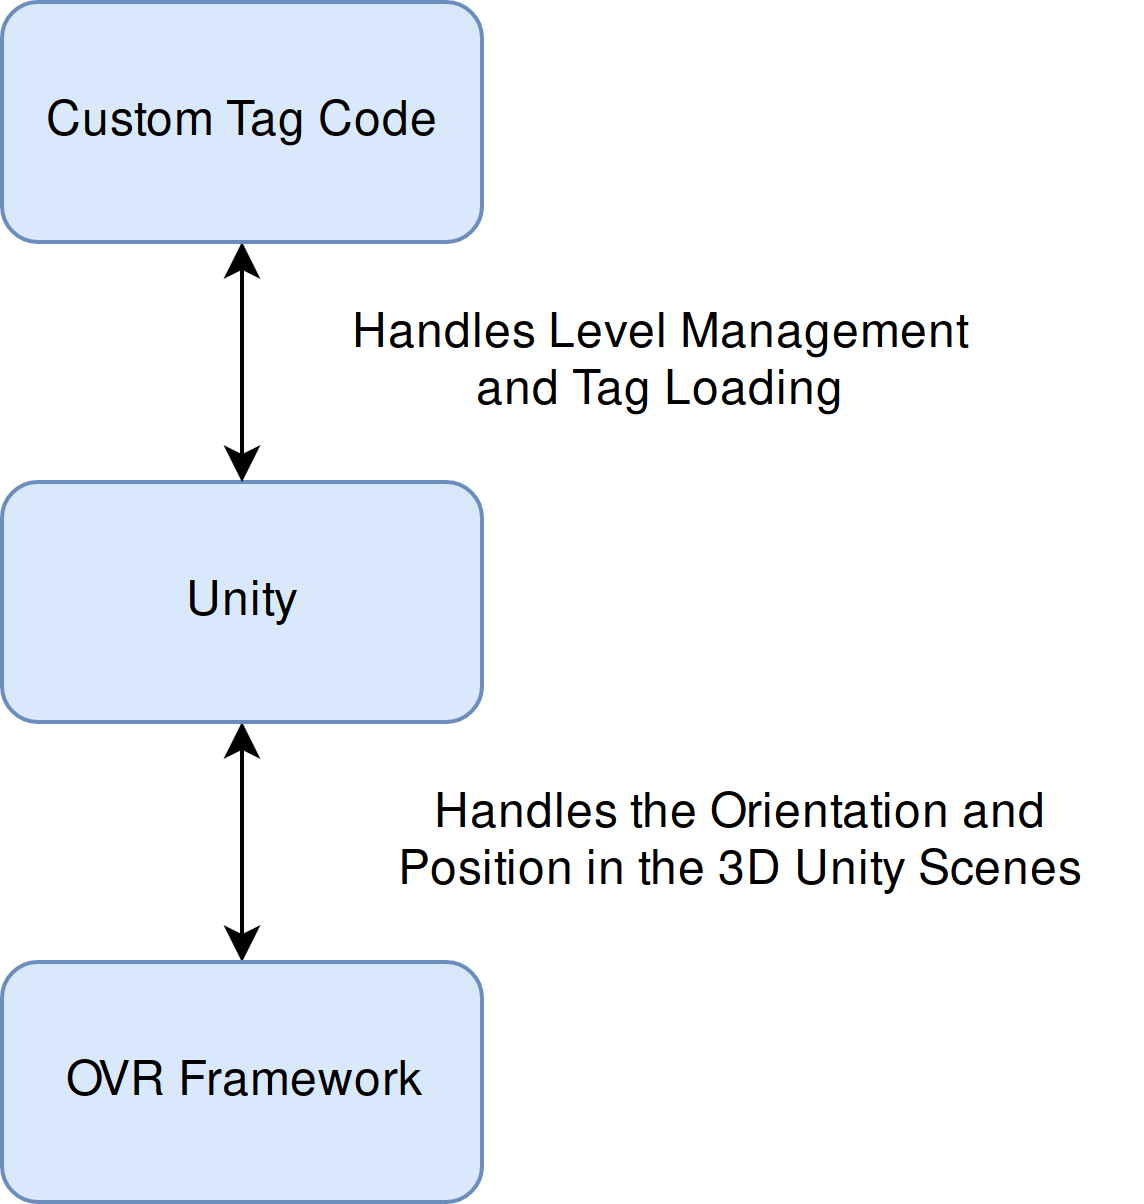
\includegraphics[height=\textwidth]{viewer_application_struct}

\subsection{Design Patterns}

Most of the design and architectural patterns we have implemented are as a
result of out choice of framework and implementation. However, any design
pattern that was not automatically included as a result of a framework as used
to ensure logical consistency and practical maintainability. It also had the
handy side effect of keeping repeated code to a minimum and allowed for rapid
iteration on the projects. This was especially helpful as the build process
would sometimes take upwards of 2 minutes and so reducing this time was crucial.

\subsubsection{VR Tagging Engine Patterns}
\begin{description}
    \item [MTV --- Model Template View] This architectural pattern is the core
        of Django and seperates the concerns of ``What data should be shown'',
        ``How the data should be shown'' and ``Which data should be shown''. It
        allows the program to scale quickly and improves iteration times by
        reducing the amount of work needed to implement a new feature down to
        the creation of a new view.

    \item [Template Methods] Django uses this behavioural pattern to great
        effect with it's class based views and they are used in this
        application to provide custom functionality with it's class based
        views. I would use the same pattern for each of the models, in that I would
        override the \inlinecode{\_\_str\_\_} method of each of the models to
        provide a string representation that is used in the administrator view
        for the application.

    \item [Adapter] Django has a set of classes known as Models which implement
        the adaptor pattern which adapts the raw SQL interface of the SQLite3
        database into a more useful python object containing many methods which
        form part of Django's object relational model. I could then use the
        adapted interface in my own code without any issue.
\end{description}

\subsubsection{VR Viewer Patterns}
\begin{description}
    \item [Entity --- Component Pattern] The Entity --- Component pattern means
        that all objects in Unity are either Entities (Unity refers to these as
        ``GameObjects'') which actually exist in the simulated space, or
        Components which are merely a method for describing a small set of
        reusable behaviors.

    \item [Composite Pattern] GameObjects in Unity follow the Composite
        pattern. This means that there is no difference between a tree-like
        structure of GameObjects and a single GameObject. This is because both
        of these are objects of the same ``GameObject'' superclass and so can
        be composed in a recursive manner. This allows for complex scenes to
        take place as nested GameObjects inherit a local coordinate space from
        their parents, meaning that 3D transformations can be stacked together
        with ease.

\end{description}

\section{Implementation}

\subsection{Development Tools}
\begin{description}
    \item[Communication] For communication with the client we will use a
        mixture of Slack messages and Email depending on the nature of the
        communication and if it needs to go on record as an official decision
        by the client.
    \item[File Sharing] For the sharing of large binary files such as Unity
        projects we will use the file sharing service ``Google Drive''. This is
        because standard version control performs very poorly when dealing with
        the large binary files usually associated with Unity projects,
        duplicating them with every revision unless they are exact duplicates
        of each other.
    \item[UI Design] The design of the Web Application's Interface will be done
        in the Django templating language (which renders out to HTML5) and
        Javascript. The design of the VR Viewer's User Interface will be done
        in the Unity Editor.
    \item[Version Control] We will use \inlinecode{git} as our primary method
        of version control as it is an industry standard with wide support for
        cloud based storage and branching.
    \item[IDE] Amartya will be using vim to write the Web Application and
        Jasper will be using the MonoDevelop to write C\# scripts for the Unity
        Application. Amartya will also use Android Studio to write a
        web-texture plugin for the VR Viewer.
    \item[Local Development Environments] Amartya will be using VirtualEnv to
        set up a easily replicable deployment environment.
\end{description}

\subsection{Front-End Technologies}
\subsubsection{VR Engine}
The front end of the VR engine was written in the Django Templating language, a
small language created by Django to allow for the creation of templates that
could render to HTML when given a specific data set which the view has
retrieved from the database. The language allows for looping constructs and
conditional operations while generating HTML so little hard-coding had to be
done to allow for multiple items and as the HTML was all generated on the
server side there is little to no need for any client side work, meaning that
the VR Tagging Engine can work from a variety of web-browsers.

However, the generated HTML could not be used for everything. In cases where a
page reload could not be afforded, such as the Tag Editor, the only solution
was to use JavaScript to forward requests such as Tag creation or deletion via
AJAX and await the server's response. But this does mean that the VR Engine is
very bandwidth efficient as all the calls can be batched up and sent to the
server in one go ensuring that duplicated data is not sent. CSS was used to
layout the app and ensure that it was visually appealing.

\subsubsection{VR Viewer}
The VR Viewer was created using Unity, a multi-platform game engine that
natively supports VR and has the ability to use native plugins. This meant that
it was perfect for creating the 3D scenes required to render the tagged VR
content as well as loading Web Content as described by the client using a
Native Plugin. The plugin was made in Android Studio and defined a class that
extended the native Android Web View, overriding the \inlinecode{onDraw} method
to render the view into a bitmap. This bitmap is then drawn into an OpenGL
texture on the plugin's main thread. Unity then defines an external texture
using the texture pointer created in the plugin and applies that texture to a
plane which is then used as a web view tag. Similar processes are applied for
all other types of tag, skipping the native plugin steps and using Unity
defined helper classes instead. Unity then handles VR input events from the
Gear VR and uses them to play/pause the video while the user is interacting
with the tags.

\subsection{Back-End Technologies}
VR Viewer lacks any persistent modifiable data and so does not really have a
back-end as such. However the VR Tagger System is a full web application using
Django and SQLite3 to handle incoming web-requests. Django was used as it is a
very elegant and popular framework written in Python, this meant that it was
not only a very simple application to write but also that it should be near
trivial to find any developer willing to work on the project and that developer
should be able to get accustomed to the environment effortlessly. SQLite3 was
chosen as it was the simplest relational database that covered all the features
that were needed, and as we do not expect to have a work load on the database
(less than 1GB in total size and fewer than 5 concurrent accesses) it should be
more than sufficient.

\subsection{Implementation of Key Functionality}
\subsection{VR Tagging System}

\begin{description}
    \item[RQ1 --- The system will have HTML5 tagging in VR space]
        When the client is pointed at a tag editor URL, e.g.\
        \url{/tagger/project/23/video/20/} which edits the video with id 20,
        which belongs to a project with id 23, the browser sends a request to
        the Django application. Which forwards the relevant data to the python
        function \inlinecode{video\_editor}.
        \begin{lstlisting}[language=Python, breaklines=true]
@login_required
def video_editor(request, project_id, video_id):
    vid = get_object_or_404(Video, id=video_id)

    if request.method == "POST":
        print(request.body)
        data = [item for item in json.loads(request.body) if "deleted" not in item]
        for item in json.loads(request.body):
            if item not in data:
                Tag.objects.filter(id=item["pk"]).delete();
        for obj in serializers.deserialize("json", json.dumps(data)):
            obj.save()
    return render(request, "tagger/video_editor.html", {"video": vid, "tags": vid.tag_set, "tags_json": serializers.serialize("json", vid.tag_set.all())})
        \end{lstlisting}
        This loads the relevant video from the Django ORM and the checks if the
        Request was a POST request. If it was it then gets the JSON that was
        sent from the client and deserializes and saves the changed tags into
        the database, deleting tags that have been marked as such, it then
        re-renders the tag editor sends this data to the user's browser as a
        response.

    \item[RQ4 --- Data structure of time indexes and coordinates kept with a
        collection\ldots]
        This mostly got changed as I realised the user didn't have to upload
        any content to the web server just to re-download it after the fact
        instead what the tags store now is something called a
        \inlinecode{remote\_url} which allows the server to know at export time
        where and what the actual file is, while still allowing the user to
        rapidly iterate on the tags having to wait on the upload process. The
        code to create these tags is shown above in the \inlinecode{video\_editor} method.

    \item[RQ11 --- Allow loading in of videos] 
        To create a new video for a project the client must first navigate to a
        project, and then to the new video page of that project. The URL is
        usually as something resembling the following
        \url{/tagger/project/23/video/new/} where 23 is the id of the project
        that the video is being uploaded to. They then fill out the form that
        they are presented with and click upload.

        Django will then dispatch them to the relevant view function

        \begin{lstlisting}[language=Python, breaklines=true]
class VideoForm(ModelForm):
    class Meta:
        model = Video
        fields = ["title", "uploaded_video", "project"]
        widgets = {"project": HiddenInput()}

def video_create(request, project_id):
    f = VideoForm(initial={"project":project_id})
    if request.method == "POST":
        f = VideoForm(request.POST, request.FILES)
        if f.is_valid():
            f.save()
            return HttpResponseRedirect("/tagger/project/{}/video/".format(project_id))
        return render(request,
                "tagger/video_detail.html",
                {"video_form": f})
    else: 
        return render(request,
                "tagger/video_detail.html",
                {"video_form": f})
        \end{lstlisting}
    A \inlinecode{VideoForm} is an python class that extends
    \inlinecode{ModelForm} a Django class that reads it's meta class to find a
    way of auto generating a form that can be used in a Django template. The
    project field is hidden as it is auto filled from the URL and the user
    should not be able to edit it directly. The form then has an is valid
    method that validates the contents of request.POST and request.FILES to
    check if they match the format given by the model. If they do then all of
    the data of the form is saved. As it is a model form this means that a
    Django object will be created with all of the settings and data from the
    request, and as the \inlinecode{FILES} object is passed in this includes
    any videos that are sent as part of a multi-part request. The user is then
    redirected to the project's video overview screen. If it is not valid then
    the user is served a refreshed page, but with a form that contains errors.
    This means that when the form is generated the errors are automatically
    included in the generated HTML with a useful CSS class. If the incoming
    request is not a post request then a request with a VideoForm is made only
    setting the project value to the incoming project id.

    \item[RQ12 --- Allow editing of custom project format] The source code also
        contains methods called \inlinecode{project\_list},
        \inlinecode{project\_create}, \inlinecode{project\_detail},
        \inlinecode{project\_delete}, \inlinecode{project\_export},
        \inlinecode{video\_list}, \inlinecode{video\_create},
        \inlinecode{video\_editor} and \inlinecode{video\_delete}. These
        functions perform the other aspects of the CRUD
        (Create/Read/Update/Destroy) that is required for the app.
\end{description}

\subsection{VR Viewer}
The VR viewer is starts by loading up the meta.xml file which is a section in
the generated project file that states what videos are included in the project,
what their tags are, if those tags are remote and so on. An example meta.xml
looks as follows.
\begin{lstlisting}[language=XML, breaklines=true]
<!-- Handy Meta File -->
<project id="24" title="Testing the File Exporter">
    <video id="21" title="Star Warz" location="project/videos/output_ke4Kqgg.webm">
        <tag remote="false" x="50" y="50" width="500" height="500" tstart="55" tend="60" local_content="Dod Gamn Stormtroopers"/>
        <tag remote="true" x="50" y="50" width="1024" height="1024" tstart="62" tend="72" remote_url="www.google.com/?q=Darth"/>
    </video>
    <video id="22" title="BBB" location="project/videos/big-buck-bunny_trailer_9RD0r16.webm">
        <tag remote="false" x="50" y="50" width="50" height="50" tstart="5" tend="7" local_content="Tree"/>
        <tag remote="false" x="50" y="50" width="50" height="50" tstart="10" tend="11" local_content="Bunny"/>
        <tag remote="false" x="50" y="50" width="60" height="60" tstart="18" tend="23" local_content="You done goofed"/>
    </video>
</project>
\end{lstlisting}
The Unity application then parses this data and uses it to create a main menu
using the New Unity GUI sub-system. This menu has a maximum video count of 20,
meaning requirement RQ18 is fulfilled. It does this by parsing the XML using
the System.XML library and extracting a list of videos. It then iterates
through the list and uses the title attribute of a video tag to generate the
necessary title for the menu button. Upon clicking this button a new scene is
loaded in which the application does several things simultaneously. It renders
the video on to a sphere fulfilling requirements RQ2, RQ5, RQ14 and RQ16. It then
re-parses the meta.xml file to get access to all of the tags under the current
video. For each tag that was created in this way, a \inlinecode{CreateTags}
script creates a prefab which contains disabled variants of all the possible
tag types. Then it performs a web-request to the remote url if the tag is a
remote one and gathers the tag type from the mime-type of the resultant file.
Otherwise the type of the tag is just text. The \inlinecode{CreateTags} script
then Instantiates clones of that prefab in all of the places were they can be
and enables the one that matched the type needed. This then proceeds to fulfil
all of the other requirements.

\subsection{Data Storage}
The data was stored in an SQLite3 database. The schema is as follows\ldots

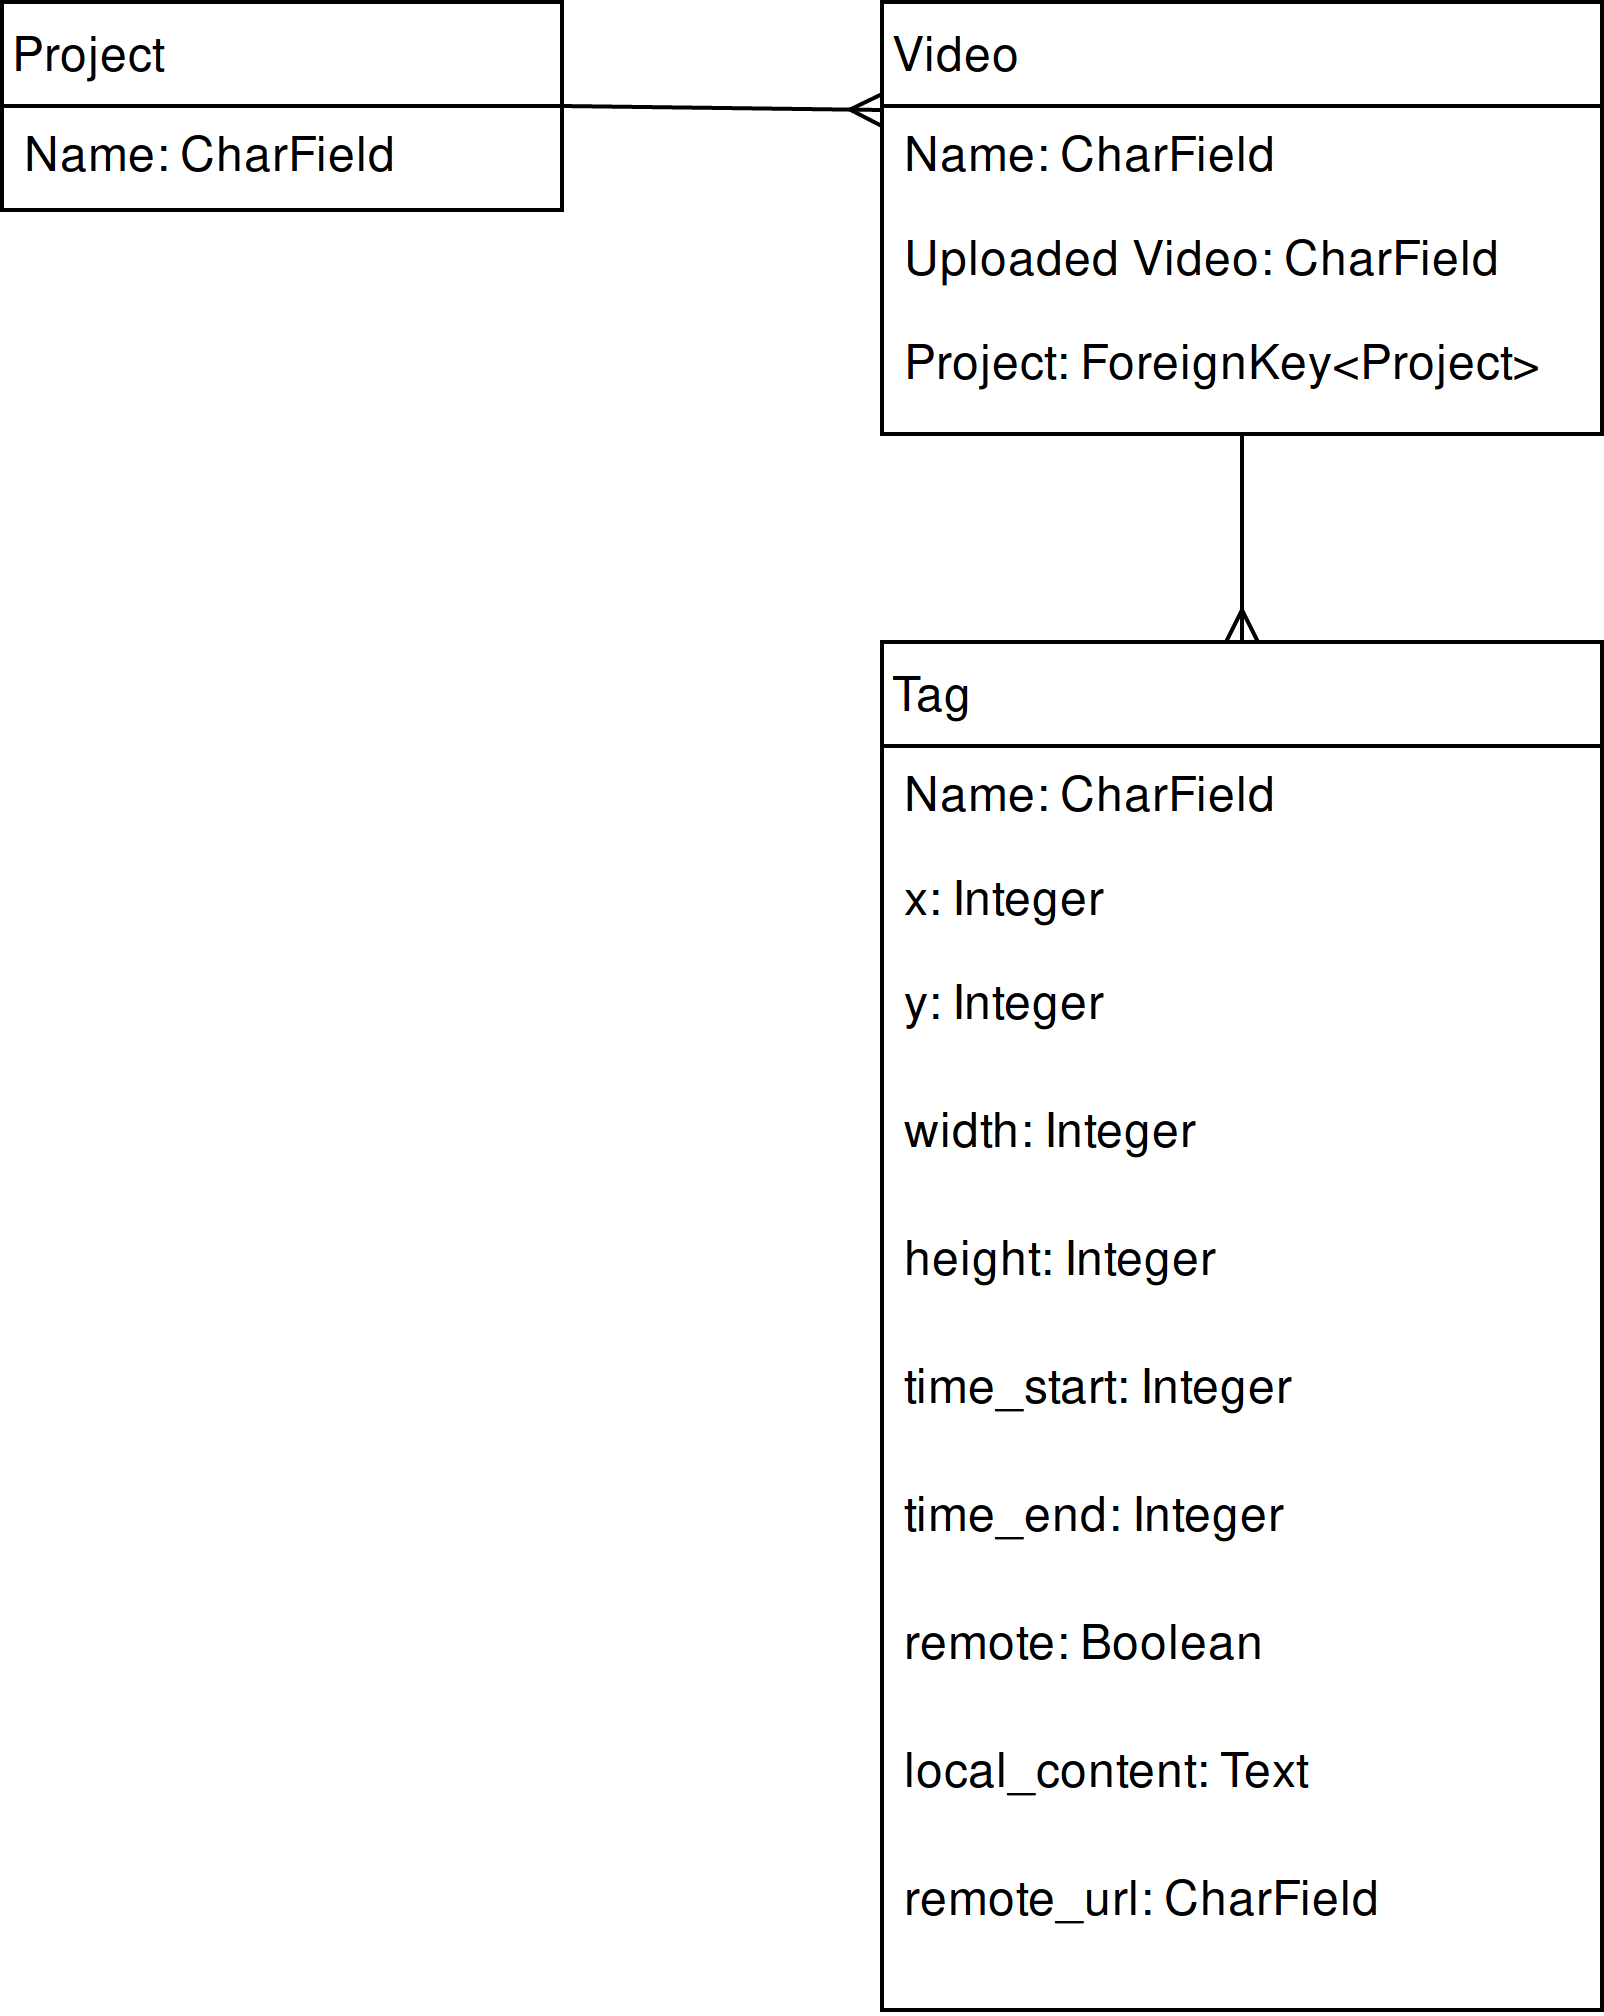
\includegraphics[height=\textwidth]{er_diagram}
\clearpage

\section{Project Management}
\chapter{Compatibility + Response Design Testing}
\end{document}
